%%%%%%%%%%%%%%%%%%%%%%%%%%%%%%%%%%%%

\section{6.4. Teste de independência de qui-quadrado}

%%%%%%%%%%%%%%%%%%%%%%%%%%%%%%%%%%%

\subsection{Crianças populares}

%%%%%%%%%%%%%%%%%%%%%%%%%%%%%%%%%%%

\begin{frame}
\frametitle{Crianças populares}
\justifying
\dq{No conjunto de dados \texttt{popular}, os alunos das 4ª a 6ª séries foram questionados se boas notas, ser atlético ou ser popular era mais importante para eles. Uma tabela de duas vias que separa os alunos por série e por escolha do fator mais importante é mostrada abaixo. Esses dados fornecem evidências para sugerir que as preferências variam de acordo com o série?
}

\twocol{0.5}{0.5}
{
\begin{center}
\begin{tabular}{rrrr}
  \hline
 & Notas & Popular & Esportes \\ 
  \hline
$4^{a}$ &  63 &  31 &  25 \\ 
$5^{a}$ &  88 &  55 &  33 \\ 
$6^{a}$ &  96 &  55 &  32 \\ 
   \hline
\end{tabular}
\end{center}
}
{
\begin{center}
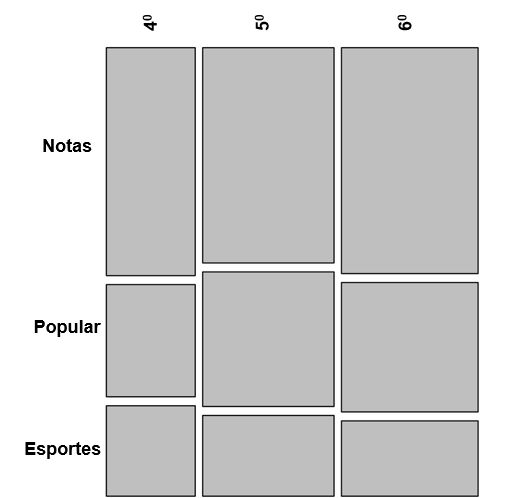
\includegraphics[width=0.8\textwidth]{6-4_chisq_indep/popular_mosaic.png}
\end{center}
}


\end{frame}

%%%%%%%%%%%%%%%%%%%%%%%%%%%%%%%%%%%

\begin{frame}
\frametitle{Teste de independência do qui-quadrado}

\begin{itemize}
\justifying
\item As hipóteses são:
\begin{itemize}
\justifying
\item[$H_0$:] A série e as preferências são independentes. As preferências não variam de acordo com a série.
\justifying
\item[$H_A$:] A série e as preferências são dependentes. As preferências variam de acordo com a série.
\end{itemize}

\pause
\justifying
\item A estatística de teste é calculada como
\[ \chi^2_{df} = \sum_{i = 1}^{k} \frac{(O - E)^2}{E} \quad \text{ onde } \quad df = (R - 1) \times (C - 1), \]
onde $k$ é o número de células, $ R $ é o número de linhas e $ C $ é o número de colunas.\\

\pause
\justifying
\item O p-valor é a área sob a curva $\chi^2_{df}$ acima da estatística de teste calculada.


\justifying
\tiny{\Note{Calculamos $df$ de forma diferente para tabelas de uma via e duas vias.}}



\end{itemize}


\end{frame}

%%%%%%%%%%%%%%%%%%%%%%%%%%%%%%%%%%%

\subsection{Contagens esperadas em tabelas de duas vias}

%%%%%%%%%%%%%%%%%%%%%%%%%%%%%%%%%%%

\begin{frame}
\frametitle{Contagens esperadas em tabelas de duas vias}
\justifying
\formula{Contagens esperadas em tabelas de duas vias}
{
\[ \text{Contagem esperada} = \frac{(\text{total da linha}) \times (\text{total da coluna})}{\text{total da tabela}} \]
}

\pause

{\small
\begin{center}
\begin{tabular}{rrrr|r}
  \hline
 & Notas & Popular & Esportes	& Total \\ 
  \hline
$4^{a}$ &  \orange{63} &  \green{31} &  25 	&119 \\ 
$5^{a}$ &  88 &  55 &  33	& 176 \\ 
$6^{a}$&  96 &  55 &  32	& 183 \\ 
   \hline
Total	& 247	& 141	& 90	& 478 \\
\end{tabular}
\end{center}
}

\pause

\[ \orange{$E_{linha~1, coluna~1} = \frac{119 \times 247}{478} = 61$} \qquad \pause
 \green{$E_{linha~1, coluna~2} = \frac{119 \times 141}{478} = 35$} \]

\end{frame}

%%%%%%%%%%%%%%%%%%%%%%%%%%%%%%%%%%%

\begin{frame}
\frametitle{Contagens esperadas em tabelas bidirecionais}
\justifying
\pq{Qual é a contagem esperada para a célula realçada?}

{\small
\begin{center}
\begin{tabular}{rrrr|r}
  \hline
 & Notas & Popular & Esportes	& Total \\ 
  \hline
$4^{a}$ &  63 &  31 &  25 	&119 \\ 
$5^{a}$ &  88 &  55 &  33   &176\\ 
$6^{a}$ &  96 &  55 &  32	& 183 \\ 
   \hline
Total	& 247	& 141	& 90	& 478 \\
\end{tabular}
\end{center}
}

\twocol{0.2}{0.8}
{
\begin{enumerate}[(a)]
\solnMult{$\frac{176 \times 141}{478}$}
\item $\frac{119 \times 141}{478}$
\item $\frac{176 \times 247}{478}$
\item $\frac{176 \times 478}{478}$
\end{enumerate}
}
{
\soln{\only<2>{\justifying
\orange{$\rightarrow$ 52\\
{\small mais do que o \# esperado de alunos do 5º ano \\
tem preferência por ser popular}}
\vspace{0.75cm}
}
}
}

\end{frame}

%%%%%%%%%%%%%%%%%%%%%%%%%%%%%%%%%%%

\begin{frame}
\frametitle{Calculando a estatística de teste em tabelas bidirecionais}
\justifying
As contagens esperadas são mostradas em \ex {azul} ao lado das contagens observadas.
\begin{center}
\begin{tabular}{rrrr|r}
  \hline
 & Notas & Popular & Esportes	& Total \\ 
  \hline
$4^{a}$ 	&  63 \ex{61} &  31 \ex{35} &  25 \ex{23}	&119 \\ 
$5^{a}$ 	&  88 \ex{91} &  55 \ex{52} &  33 \ex{33}	& 176 \\ 
$6^{a}$	&  96 \ex{95} &  55 \ex{54} &  32 \ex{34}	& 183 \\ 
   \hline
Total	& 247	& 141	& 90	& 478 \\
\end{tabular}
\end{center}

\vspace{0.5cm}

\pause

\begin{eqnarray*} 
\chi^2 &=& \sum \frac{(63 - 61)^2}{61} + \frac{(31 - 35)^2}{35} + \cdots + \frac{(32 - 34)^2}{34} = 1.3121 \\
\pause
df &=& (R - 1) \times (C - 1) = (3 - 1) \times (3 - 1) = 2 \times 2 = 4 
\end{eqnarray*}

\end{frame}

%%%%%%%%%%%%%%%%%%%%%%%%%%%%%%%%%%%

\subsection{Resultados}

%%%%%%%%%%%%%%%%%%%%%%%%%%%%%%%%%%%

\begin{frame}
\frametitle{Calculando o p-valor}
\justifying
\pq{Qual dos seguintes é o p-valor correto para este teste de hipóteses?
\[ \chi^2 = 1.3121 \qquad df = 4 \]
}

\twocol{0.6}{0.4}{
\begin{center}
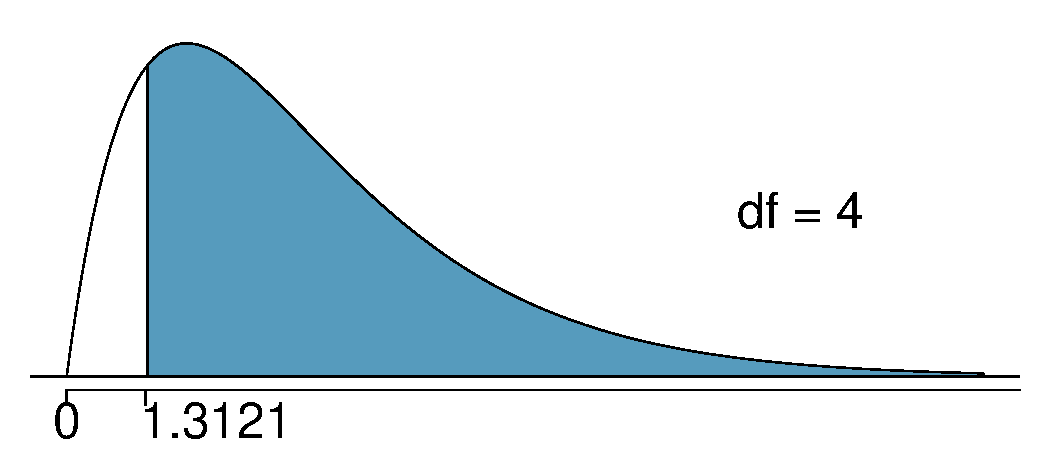
\includegraphics[width=0.67\textwidth]{6-4_chisq_indep/popular.pdf}
\end{center}
}
{
{\small
\begin{enumerate}[(a)]
\setlength{\itemsep}{0in}
\solnMult{ maior que 0.3}
\item entre 0.3 e 0.2
\item entre 0.2 e 0.1
\item entre 0.1 e 0.05
\item menor que 0.001
\end{enumerate}
}
}
\end{frame}
%%%%%%%%%%%%%%%%%%%%%%%%%%%%%%%%%%%

\begin{frame}
\frametitle{Calculando o p-valor}

\begin{center}
{\scriptsize
\begin{tabular}{r | rrrr | rrrr |}
  \hline
Cauda superior & 0.3 & 0.2 & 0.1 & 0.05 & 0.02 & 0.01 & 0.005 & 0.001 \\ 
  \hline
df \hfill 1 &  1.07 &  1.64 &  2.71 &  3.84 &  5.41 &  6.63 &  7.88 &  10.83 \\ 
  2 &  2.41 &  3.22 &  4.61 &  5.99 &  7.82 &  9.21 &  10.60 &  13.82 \\ 
  3 &  3.66 &  4.64 &  6.25 &  7.81 &  9.84 &  11.34 &  12.84 &  16.27 \\ 
  4 &  4.88 &  5.99 &  7.78 &  9.49 &  11.67 &  13.28 &  14.86 &  18.47 \\ 
  5 &  6.06 &  7.29 &  9.24 &  11.07 &  13.39 &  15.09 &  16.75 &  20.52 \\ 
\end{tabular}
}
\end{center}

\end{frame}

%%%%%%%%%%%%%%%%%%%%%%%%%%%%%%%%%%%

\begin{frame}
\frametitle{Conclusão}
\justifying
\dq{Esses dados fornecem evidências para sugerir que as preferências variam de acordo com a série?}

\begin{itemize}
\justifying
\item[$H_0$:] A série e as preferências são independentes. As preferências não variam de acordo com a séries.
\justifying
\item[$H_A$:] A série e as preferências são dependentes. As preferências variam de acordo com a série. \\

\end{itemize}

$\:$ \\
\justifying
\soln{\only<2>{Como o p-valor é alto, não rejeitamos $H_0$. Os dados não fornecem evidências convincentes de que a série e as preferências são dependentes. Não parece que as preferências variam por série.
}
}

\end{frame}